\section{Sistema de proteção contra descargas atmosféricas e aterramento} \label{section: SPDA-ATT}

De acordo com \cite{mattostecnicas}, os termos referência elétrica, massa condutora e terra são tratados coloquialmente como aterramento. O autor segue explicando que a principal razão para aterrar um sistema surge da necessidade de proteger as pessoas contra choques originados nas instalações elétricas.

Devemos extrapolar as proteções de um sistemas de aterramento combinando  com um SPDA, ampliando desta forma as medidas de proteção para  atuarem em edificações contra a descarga de raios, com o objetivo de evitar ou minimizar os danos que possam ser causados à própria edificação, como a ocorrência de incêndios e explosões, além dos danos à integridade física das pessoas que se encontrem dentro ou no perímetro da edificação.

% Copy this to add more chapters
\subsection{Generalidades} \label{subsection: SPDA-ATT-general}

XXXXXXXXXXXXXXXXXXXXXXXXXXXXXXXXXXXXXXXXXX

% Copy this to add more chapters
%\subsubsection{Generalidades} \label{lighting - generalidades}

\begin{enumerate}
	
	\item O projeto de iluminação deverá abranger, onde cabível, os seguintes sistemas:
	\begin{enumerate}
		\item Iluminação geral de interiores
		\item Iluminação externa
		\item Iluminação específica
		\item Iluminação de emergência
		\item Iluminação de sinalização e luz de obstáculos
		\item Iluminação cênica (quando esta for exigida)
	\end{enumerate}
	
	\item Não será aceita a utilização de eletrodutos de bitola menor que 3/4” de diâmetro para iluminação.
	
	\item Poderá ser considerada a instalação como previsão de reserva, eletrodutos com bitolas superiores às necessárias para as bitolas iniciais dos condutores ou eletrodutos vazios.
	
	\item O projeto deverá priorizar, sempre que possível, a utilização de luminárias energeticamente eficientes.
	
	\item O projeto sempre deverá priorizar a utilização de equipamentos e materiais facilmente encontrados no mercado.
	
	\item Deverá ser priorizada a utilização de luminárias na seguinte ordem:\label{light: tipo1}
	\begin{enumerate}
		\item Utilização de luminárias LED com lâmpadas TUBOLED modelo T5, dado que as lâmpadas são facilmente substituídas.

		\item Luminárias com lâmpadas LED (a lâmpada ou o conjunto de lâmpadas pode ser facilmente substituído);
		
		\item Luminárias LED (o conjunto de LEDs não pode ser substituído, entretanto o \textit{driver} pode ser substituído;
	\end{enumerate}

	\item Deverá ser evitada, entretanto poderá ser utilizada em casos excepcionais:\label{light: tipo2}
	\begin{enumerate} 
		
		\item Luminárias LED cujo conjunto de lâmpadas e driver não podem ser substituídos (a manutenção deverá trocar todo o conjunto em caso de defeito)		
	\end{enumerate}

	\item Casos que não se enquadrem nos itens \ref{light: tipo1} e \ref{light: tipo2}, a contratante deverá ser contatada para definir junto a contratada quais luminárias e lâmpadas serão utilizadas.

	
	\item O projeto de iluminação atenderá aos níveis de iluminamento necessários em cada ambiente de acordo com a NBR-8.995 e determinará o tipo de iluminação, número de lâmpadas por luminárias, número e tipo de luminária, detalhes de montagem, localização das luminárias, caixas de passagem e interruptores, caminhamento dos condutores e tipo para sua instalação. 
	
	\item Para o projeto de iluminação poderão ser adotados os valores mínimos dos níveis de iluminamento recomendados pelas NBR 8.995. O tipo de fonte luminosa e da luminária e a sua distribuição no local deverão ser harmonizados com os projetos de arquitetura e aprovados pela coordenação do desenvolvimento do projeto.
	
	\item \label{lighting: bitola minima} Para circuitos de iluminação, será adotado a bitola mínima de 2,5mm\textsuperscript{2} observando-se, entretanto, a diferenciação de cores nas respectivas fiações.
	
	\item As derivações para a alimentação das luminárias serão executadas utilizando-se cabos de cobre “PP” de 3 vias \#1,5mm\textsuperscript{2} devendo ser indicadas em nota e preferencialmente em detalhe de projeto;
	
	\item Em instalações aparentes deverá ser utilizada as linhas disponíveis da Wetzel como referência técnica para interruptores e tampas montados em conduletes de alumínio
	
	\item A contratante utiliza alguns modelos de luminária (interna, externa e pública) como padrão de referência técnica. O projetista deverá consultar o apêndice XXXXXX para obter estes modelos ou apresentar à Engenharia da contratante para aprovação os modelos com características similares que pretende utilizar no projeto.
	
	\item Ao dimensionar os eletrodutos de tomadas, os mesmos deverão ser dimensionados com bitola mínima de 3/4"%$\dfrac{3}{4}$"
\end{enumerate}

% Copy this to add more chapters
%\subsubsection{Iluminação de interiores}\label {section: iluminacao_interiores}
	\begin{enumerate}
		\item Para a correta localização das fontes luminosas, a contratada, sempre que possível disporá as luminárias de forma simétrica a fim de garantir um bom bom fator de uniformidade (vide exemplo na figura \ref*{fig: disposicao}). Quaisquer disposições em contrário, a fiscalização deverá ser consultada.
		\begin{figure}[H]
			\centering
			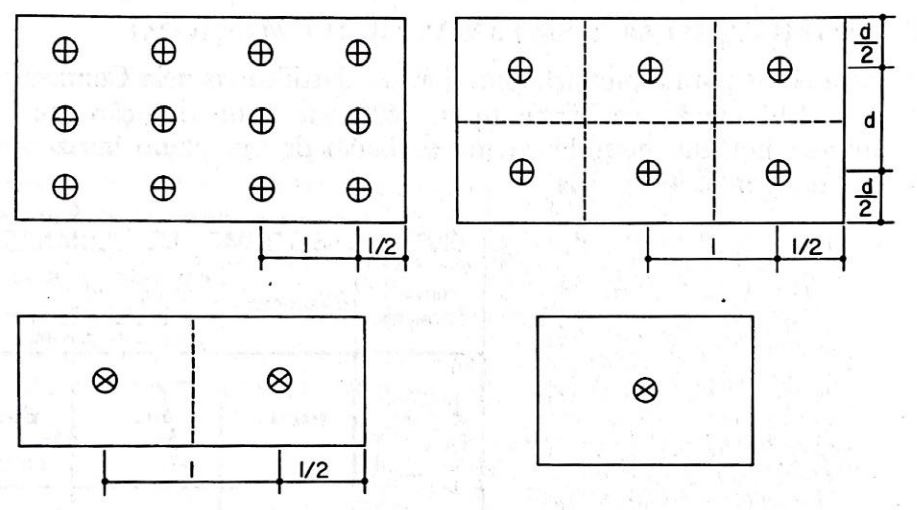
\includegraphics[width=\textwidth]{Figures/3. Lighting/light-disposicao.jpg}
			\hfill
			\caption{Disposição típicas de montagem para luminárias de iluminação de interior}  Referência \cite{de1987iluminação} p.112
			\label{fig: disposicao}
		\end{figure}
		
		\item Em instalações embutidas deverá ser utilizada a linha "PIALPLUS" da Legrand como referência técnica para interruptores e tampas
		
		\item Em instalações aparentes deverá ser utilizada a linha "Condulete TOP" da Tigre ou as linhas disponíveis da Wetzel como referência técnica para interruptores e tampas montados em conduletes de PVC
		
		\item Em instalações aparentes deverá ser utilizada as linhas disponíveis da Wetzel como referência técnica para interruptores e tampas montados em conduletes de alumínio
		
		\item\label{light:wc1}Em circuito de iluminação de banheiros e lavábulos será permitido conectar tomadas de uso geral (até 2 tomadas de 200W) ao referido circuito.
		
		\item\label{light:wc2}Em circuito de iluminação de banheiros e lavábulos será permitido conectar renovadores de ar do tipo "ventokit".
		
		\item Tomadas de uso geral não podem ser conectadas a circuitos de iluminação, a exceção das preconizadas nos itens \ref*{light:wc1} e \ref*{light:wc2}
		
		\item Em biotérios a contratada deverá prever um sistema de iluminação totalmente dimerizável
		
		\item Em Laboratórios NB3 ou NBA3 as luminárias dimensionadas serão do tipo herméricas
		\begin{enumerate}
			\item Laboratórios NB3 ou NBA3 com pavimento técnico a contratada deverá prever a remoção ou substituição dos equipamentos pelo referido pavimento, indicando em detalhe de projeto e notas
			\item Laboratórios NB3 ou NBA3 sem pavimento técnico e com forro de gesso, a contratada deverá prever em projeto que a face que possui o difusor da luminária irá facear o gesso e garantir a estanqueidade da área por sobre o gesso quando for necessário efetuar a manutenção da mesma.
			\item Demais casos deverão ser analisados pela contratada e discutidos com a Engenharia da COGIC.
		\end{enumerate}

		\item\label{light:encaixe10A}Nos caso dos encaixes rápidos utilizarem o conjunto tomada/plugue, deverá ser utilizada uma tomada de 10A
		
		\item As luminárias deverão ser projetadas tendo-se em mente a utilização de engate-rápido através de plugues e tomadas, ou dispositivos equivalentes, devendo a mesma ser indicada em nota e detalhada em projeto. Dois exemplos a seguir.
		
		\begin{figure}[H]
			\centering
			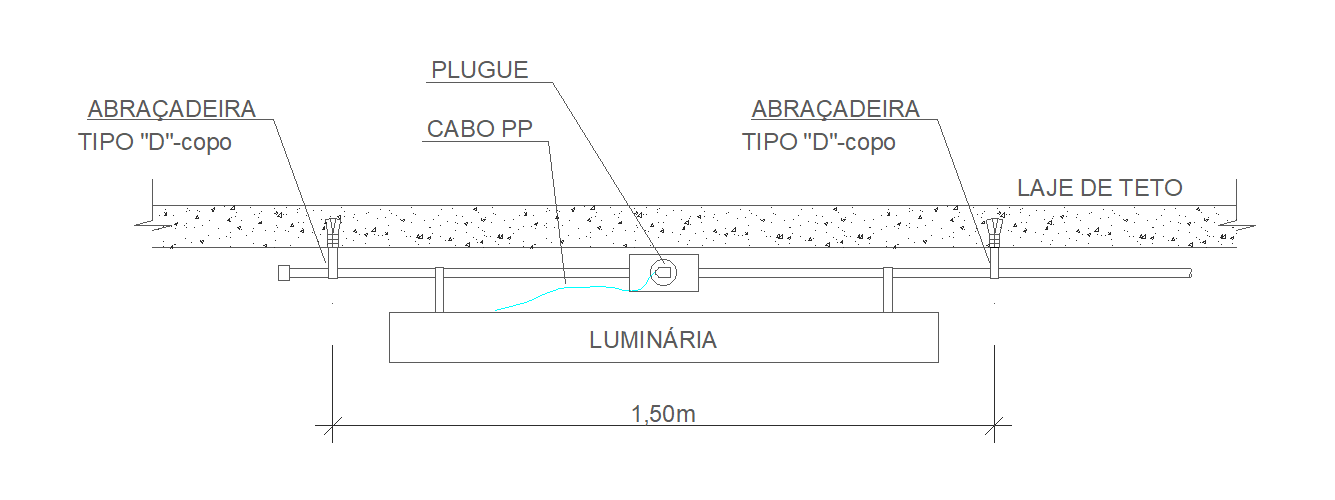
\includegraphics[width=\textwidth]{Figures/3. Lighting/light-engate rapido1.png}
			\hfill
			\caption{Encaixe rápido usando condulete e plugue de tomada ex.1}
			\label{fig: engate-rapido1}
		\end{figure}
		\begin{figure}[H]
			\centering
			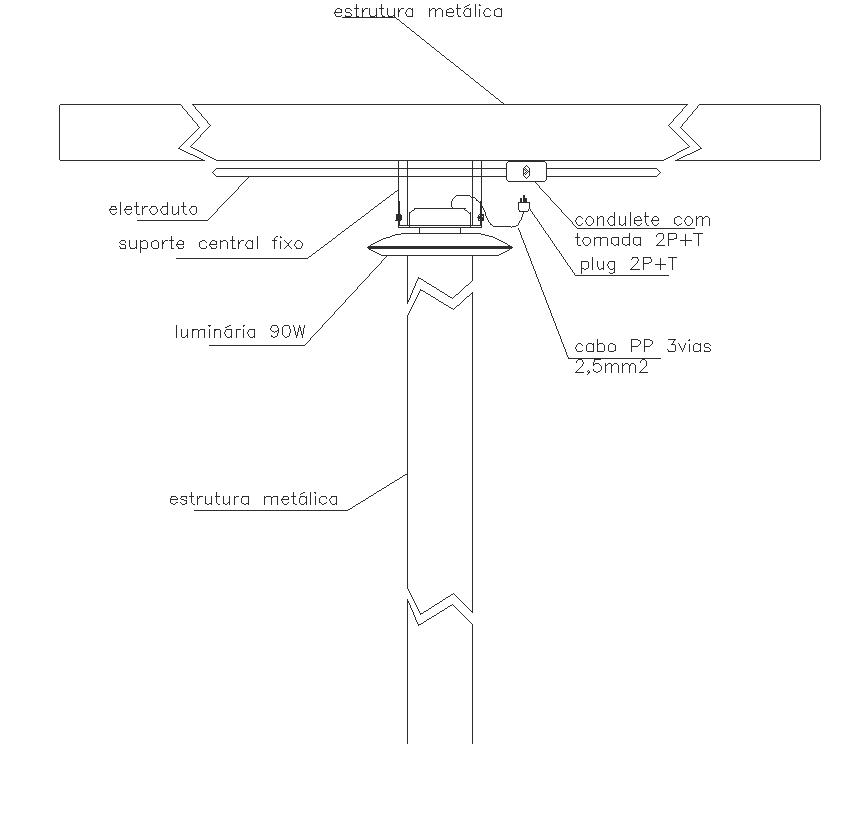
\includegraphics[scale=0.25]{Figures/3. Lighting/light-engate rapido2.png}
			\hfill
			\caption{Encaixe rápido usando condulete e plugue de tomada ex. 2}
			\label{fig: engate-rapido2}
		\end{figure}


		\item Luminárias instaladas em corredores deverão ser instaladas no sentido longitudinal a fim de obter um melhor rendimento no brilho e evitar ofuscamento. Melhores referências e explicações pode ser obtidas em \cite{simons2008lighting} p.74-75 e \cite{van2019interior} p.413.
		
		\item Luminárias em corredores só poderão ser instaladas no sentido transversal caso alguma exceção impossibilite a montagem no sentido longitudinal
	
	\end{enumerate}

% Copy this to add more chapters
%\subsubsection{Iluminação de emergência e sinalização de obstáculos}


	\paragraph*{Locais de instalação}
	
	Os locais específicos onde se fazem necessária a instalação de sinalização de emergência são:
	
	\begin{figure}[H]
		\centering
		\begin{subfigure}[b]{0.3\textwidth}
			\centering
			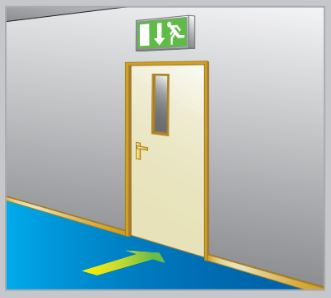
\includegraphics[width=\textwidth]{Figures/3. Lighting/light-safety1.jpg}
			\caption{A cada porta de emergência}
			\label{fig: style 1 image a}
		\end{subfigure}
		\hfill
		\begin{subfigure}[b]{0.3\textwidth}
			\centering
			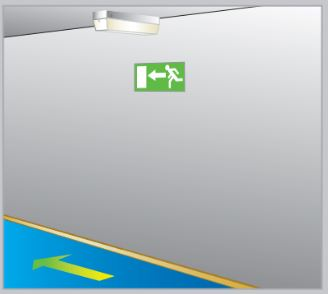
\includegraphics[width=\textwidth]{Figures/3. Lighting/light-safety2.jpg}
			\caption{Todas as sinalizações de saída}
			\label{fig: style 1 image b}
		\end{subfigure}
		\hfill
		\begin{subfigure}[b]{0.3\textwidth}
			\centering
			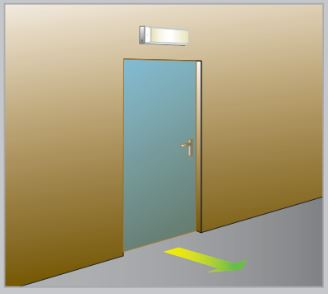
\includegraphics[width=\textwidth]{Figures/3. Lighting/light-safety3.jpg}
			\caption{Nas saídas de emergência}
			\label{fig: style 1 image c}
		\end{subfigure}
	\end{figure}

	\begin{figure}[H]
		\centering
		\begin{subfigure}[b]{0.3\textwidth}
			\centering
			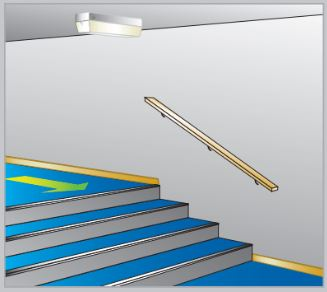
\includegraphics[width=\textwidth]{Figures/3. Lighting/light-safety4.jpg}
			\caption{Próximo escadas}
			\label{fig: style 1 image d}
		\end{subfigure}
		\hfill
		\begin{subfigure}[b]{0.3\textwidth}
			\centering
			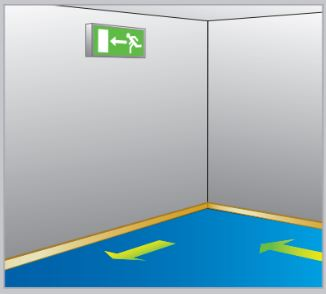
\includegraphics[width=\textwidth]{Figures/3. Lighting/light-safety5.jpg}
			\caption{Nas mudanças de direção}
			\label{fig: style 1 image e}
		\end{subfigure}
		\hfill
		\begin{subfigure}[b]{0.3\textwidth}
			\centering
			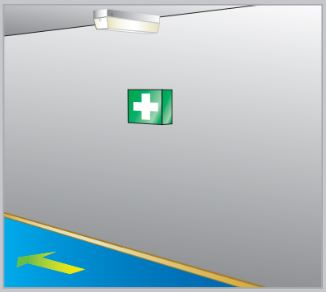
\includegraphics[width=\textwidth]{Figures/3. Lighting/light-safety6.jpg}
			\caption{Nos pontos de primeiro socorros}
			\label{fig: style 1 image f}
		\end{subfigure}
	\end{figure}

	\begin{figure}[H]
		\centering
		\begin{subfigure}[b]{0.3\textwidth}
			\centering
			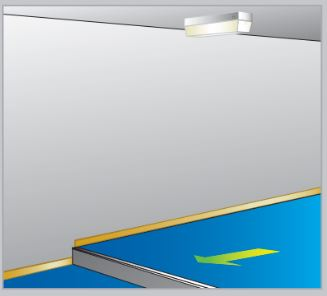
\includegraphics[width=\textwidth]{Figures/3. Lighting/light-safety7.jpg}
			\caption{A cada mudança de nível}
			\label{fig: style 1 image g}
		\end{subfigure}
		\hfill
		\begin{subfigure}[b]{0.3\textwidth}
			\centering
			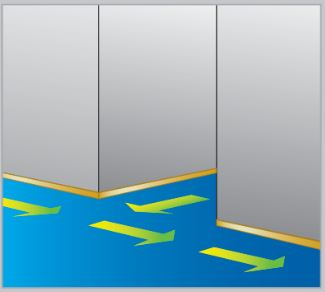
\includegraphics[width=\textwidth]{Figures/3. Lighting/light-safety8.jpg}
			\caption{Nas intersecções dos corredores}
			\label{fig: style 1 image h}
		\end{subfigure}
		\hfill
		\begin{subfigure}[b]{0.3\textwidth}
			\centering
			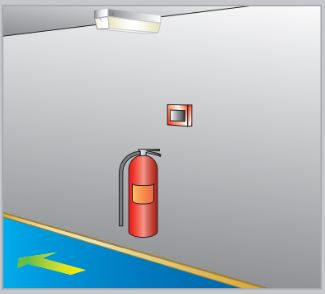
\includegraphics[width=\textwidth]{Figures/3. Lighting/light-safety9.jpg}
			\caption{Próximo a equipamentos de extinção de incêndio}
			\label{fig: style 1 image y}
		\end{subfigure}
		\caption{Localização das luminárias de emergência} fonte das imagens \cite{eaton2013} 
		\label{fig: safety-luminarires-places}
	\end{figure}




% Copy this to add more chapters
\subsection{Aterramento} \label{subsection: grounding}

XXXXXXXXXXXXXXXXXXXXXXXXXXXXXXXXXXXXXXXXXX

% Copy this to add more chapters
%\subsubsection{Generalidades} \label{lighting - generalidades}

\begin{enumerate}
	
	\item O projeto de iluminação deverá abranger, onde cabível, os seguintes sistemas:
	\begin{enumerate}
		\item Iluminação geral de interiores
		\item Iluminação externa
		\item Iluminação específica
		\item Iluminação de emergência
		\item Iluminação de sinalização e luz de obstáculos
		\item Iluminação cênica (quando esta for exigida)
	\end{enumerate}
	
	\item Não será aceita a utilização de eletrodutos de bitola menor que 3/4” de diâmetro para iluminação.
	
	\item Poderá ser considerada a instalação como previsão de reserva, eletrodutos com bitolas superiores às necessárias para as bitolas iniciais dos condutores ou eletrodutos vazios.
	
	\item O projeto deverá priorizar, sempre que possível, a utilização de luminárias energeticamente eficientes.
	
	\item O projeto sempre deverá priorizar a utilização de equipamentos e materiais facilmente encontrados no mercado.
	
	\item Deverá ser priorizada a utilização de luminárias na seguinte ordem:\label{light: tipo1}
	\begin{enumerate}
		\item Utilização de luminárias LED com lâmpadas TUBOLED modelo T5, dado que as lâmpadas são facilmente substituídas.

		\item Luminárias com lâmpadas LED (a lâmpada ou o conjunto de lâmpadas pode ser facilmente substituído);
		
		\item Luminárias LED (o conjunto de LEDs não pode ser substituído, entretanto o \textit{driver} pode ser substituído;
	\end{enumerate}

	\item Deverá ser evitada, entretanto poderá ser utilizada em casos excepcionais:\label{light: tipo2}
	\begin{enumerate} 
		
		\item Luminárias LED cujo conjunto de lâmpadas e driver não podem ser substituídos (a manutenção deverá trocar todo o conjunto em caso de defeito)		
	\end{enumerate}

	\item Casos que não se enquadrem nos itens \ref{light: tipo1} e \ref{light: tipo2}, a contratante deverá ser contatada para definir junto a contratada quais luminárias e lâmpadas serão utilizadas.

	
	\item O projeto de iluminação atenderá aos níveis de iluminamento necessários em cada ambiente de acordo com a NBR-8.995 e determinará o tipo de iluminação, número de lâmpadas por luminárias, número e tipo de luminária, detalhes de montagem, localização das luminárias, caixas de passagem e interruptores, caminhamento dos condutores e tipo para sua instalação. 
	
	\item Para o projeto de iluminação poderão ser adotados os valores mínimos dos níveis de iluminamento recomendados pelas NBR 8.995. O tipo de fonte luminosa e da luminária e a sua distribuição no local deverão ser harmonizados com os projetos de arquitetura e aprovados pela coordenação do desenvolvimento do projeto.
	
	\item \label{lighting: bitola minima} Para circuitos de iluminação, será adotado a bitola mínima de 2,5mm\textsuperscript{2} observando-se, entretanto, a diferenciação de cores nas respectivas fiações.
	
	\item As derivações para a alimentação das luminárias serão executadas utilizando-se cabos de cobre “PP” de 3 vias \#1,5mm\textsuperscript{2} devendo ser indicadas em nota e preferencialmente em detalhe de projeto;
	
	\item Em instalações aparentes deverá ser utilizada as linhas disponíveis da Wetzel como referência técnica para interruptores e tampas montados em conduletes de alumínio
	
	\item A contratante utiliza alguns modelos de luminária (interna, externa e pública) como padrão de referência técnica. O projetista deverá consultar o apêndice XXXXXX para obter estes modelos ou apresentar à Engenharia da contratante para aprovação os modelos com características similares que pretende utilizar no projeto.
	
	\item Ao dimensionar os eletrodutos de tomadas, os mesmos deverão ser dimensionados com bitola mínima de 3/4"%$\dfrac{3}{4}$"
\end{enumerate}

% Copy this to add more chapters
%\subsubsection{Iluminação de interiores}\label {section: iluminacao_interiores}
	\begin{enumerate}
		\item Para a correta localização das fontes luminosas, a contratada, sempre que possível disporá as luminárias de forma simétrica a fim de garantir um bom bom fator de uniformidade (vide exemplo na figura \ref*{fig: disposicao}). Quaisquer disposições em contrário, a fiscalização deverá ser consultada.
		\begin{figure}[H]
			\centering
			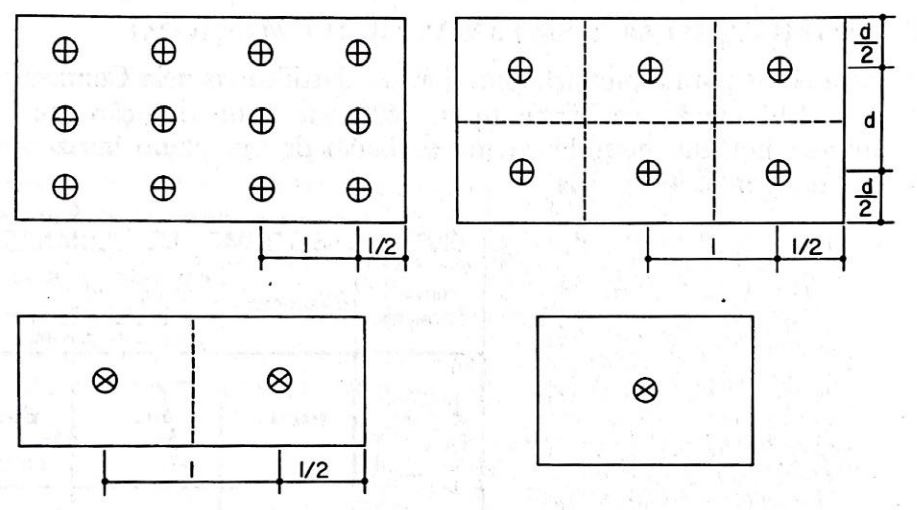
\includegraphics[width=\textwidth]{Figures/3. Lighting/light-disposicao.jpg}
			\hfill
			\caption{Disposição típicas de montagem para luminárias de iluminação de interior}  Referência \cite{de1987iluminação} p.112
			\label{fig: disposicao}
		\end{figure}
		
		\item Em instalações embutidas deverá ser utilizada a linha "PIALPLUS" da Legrand como referência técnica para interruptores e tampas
		
		\item Em instalações aparentes deverá ser utilizada a linha "Condulete TOP" da Tigre ou as linhas disponíveis da Wetzel como referência técnica para interruptores e tampas montados em conduletes de PVC
		
		\item Em instalações aparentes deverá ser utilizada as linhas disponíveis da Wetzel como referência técnica para interruptores e tampas montados em conduletes de alumínio
		
		\item\label{light:wc1}Em circuito de iluminação de banheiros e lavábulos será permitido conectar tomadas de uso geral (até 2 tomadas de 200W) ao referido circuito.
		
		\item\label{light:wc2}Em circuito de iluminação de banheiros e lavábulos será permitido conectar renovadores de ar do tipo "ventokit".
		
		\item Tomadas de uso geral não podem ser conectadas a circuitos de iluminação, a exceção das preconizadas nos itens \ref*{light:wc1} e \ref*{light:wc2}
		
		\item Em biotérios a contratada deverá prever um sistema de iluminação totalmente dimerizável
		
		\item Em Laboratórios NB3 ou NBA3 as luminárias dimensionadas serão do tipo herméricas
		\begin{enumerate}
			\item Laboratórios NB3 ou NBA3 com pavimento técnico a contratada deverá prever a remoção ou substituição dos equipamentos pelo referido pavimento, indicando em detalhe de projeto e notas
			\item Laboratórios NB3 ou NBA3 sem pavimento técnico e com forro de gesso, a contratada deverá prever em projeto que a face que possui o difusor da luminária irá facear o gesso e garantir a estanqueidade da área por sobre o gesso quando for necessário efetuar a manutenção da mesma.
			\item Demais casos deverão ser analisados pela contratada e discutidos com a Engenharia da COGIC.
		\end{enumerate}

		\item\label{light:encaixe10A}Nos caso dos encaixes rápidos utilizarem o conjunto tomada/plugue, deverá ser utilizada uma tomada de 10A
		
		\item As luminárias deverão ser projetadas tendo-se em mente a utilização de engate-rápido através de plugues e tomadas, ou dispositivos equivalentes, devendo a mesma ser indicada em nota e detalhada em projeto. Dois exemplos a seguir.
		
		\begin{figure}[H]
			\centering
			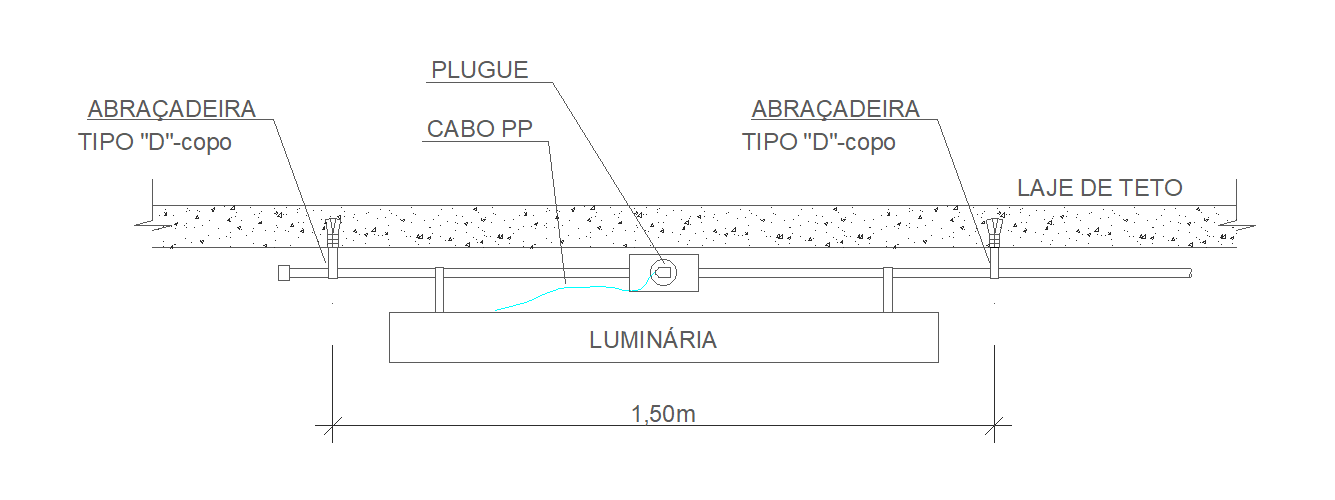
\includegraphics[width=\textwidth]{Figures/3. Lighting/light-engate rapido1.png}
			\hfill
			\caption{Encaixe rápido usando condulete e plugue de tomada ex.1}
			\label{fig: engate-rapido1}
		\end{figure}
		\begin{figure}[H]
			\centering
			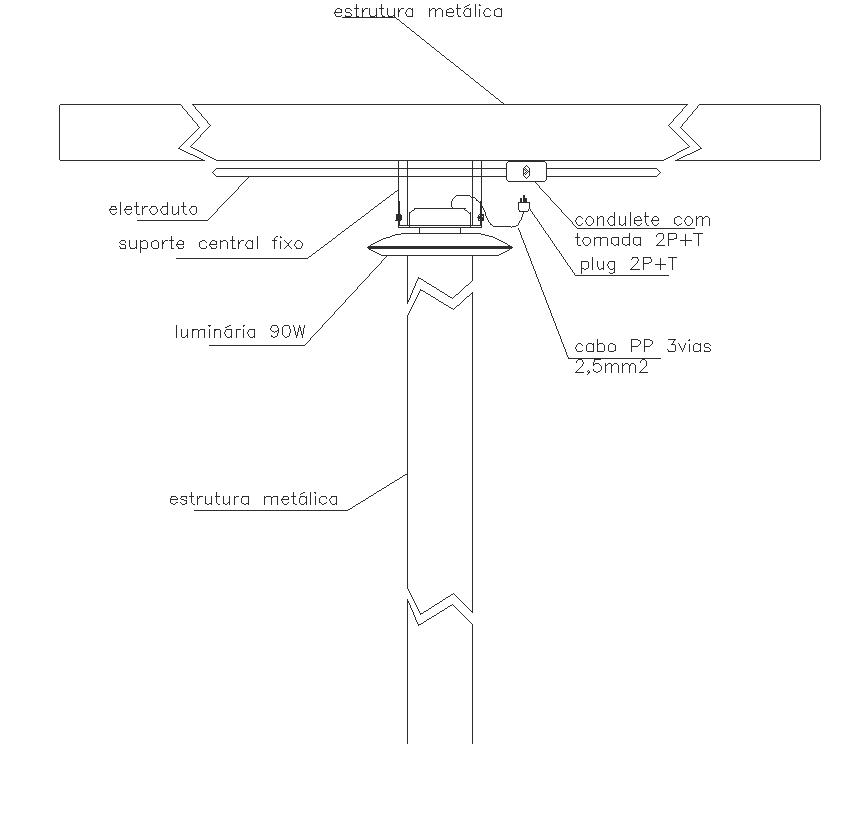
\includegraphics[scale=0.25]{Figures/3. Lighting/light-engate rapido2.png}
			\hfill
			\caption{Encaixe rápido usando condulete e plugue de tomada ex. 2}
			\label{fig: engate-rapido2}
		\end{figure}


		\item Luminárias instaladas em corredores deverão ser instaladas no sentido longitudinal a fim de obter um melhor rendimento no brilho e evitar ofuscamento. Melhores referências e explicações pode ser obtidas em \cite{simons2008lighting} p.74-75 e \cite{van2019interior} p.413.
		
		\item Luminárias em corredores só poderão ser instaladas no sentido transversal caso alguma exceção impossibilite a montagem no sentido longitudinal
	
	\end{enumerate}

% Copy this to add more chapters
%\subsubsection{Iluminação de emergência e sinalização de obstáculos}


	\paragraph*{Locais de instalação}
	
	Os locais específicos onde se fazem necessária a instalação de sinalização de emergência são:
	
	\begin{figure}[H]
		\centering
		\begin{subfigure}[b]{0.3\textwidth}
			\centering
			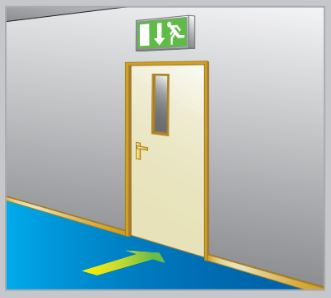
\includegraphics[width=\textwidth]{Figures/3. Lighting/light-safety1.jpg}
			\caption{A cada porta de emergência}
			\label{fig: style 1 image a}
		\end{subfigure}
		\hfill
		\begin{subfigure}[b]{0.3\textwidth}
			\centering
			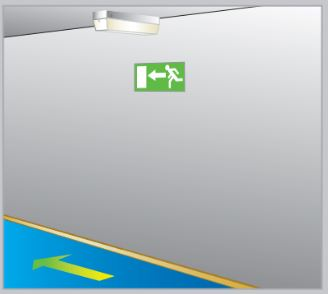
\includegraphics[width=\textwidth]{Figures/3. Lighting/light-safety2.jpg}
			\caption{Todas as sinalizações de saída}
			\label{fig: style 1 image b}
		\end{subfigure}
		\hfill
		\begin{subfigure}[b]{0.3\textwidth}
			\centering
			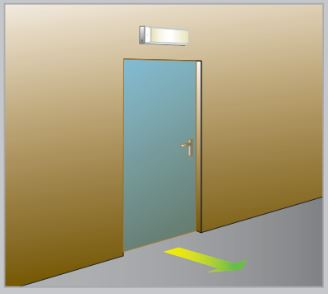
\includegraphics[width=\textwidth]{Figures/3. Lighting/light-safety3.jpg}
			\caption{Nas saídas de emergência}
			\label{fig: style 1 image c}
		\end{subfigure}
	\end{figure}

	\begin{figure}[H]
		\centering
		\begin{subfigure}[b]{0.3\textwidth}
			\centering
			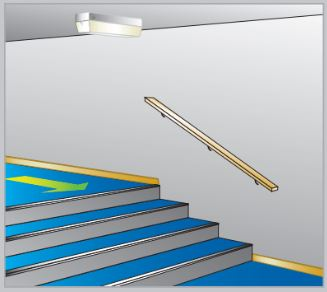
\includegraphics[width=\textwidth]{Figures/3. Lighting/light-safety4.jpg}
			\caption{Próximo escadas}
			\label{fig: style 1 image d}
		\end{subfigure}
		\hfill
		\begin{subfigure}[b]{0.3\textwidth}
			\centering
			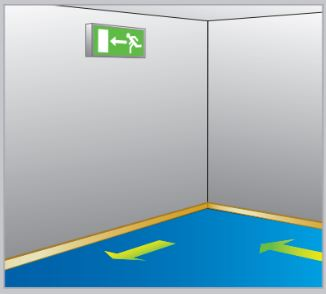
\includegraphics[width=\textwidth]{Figures/3. Lighting/light-safety5.jpg}
			\caption{Nas mudanças de direção}
			\label{fig: style 1 image e}
		\end{subfigure}
		\hfill
		\begin{subfigure}[b]{0.3\textwidth}
			\centering
			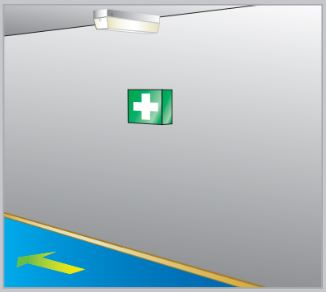
\includegraphics[width=\textwidth]{Figures/3. Lighting/light-safety6.jpg}
			\caption{Nos pontos de primeiro socorros}
			\label{fig: style 1 image f}
		\end{subfigure}
	\end{figure}

	\begin{figure}[H]
		\centering
		\begin{subfigure}[b]{0.3\textwidth}
			\centering
			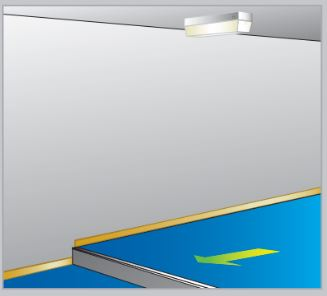
\includegraphics[width=\textwidth]{Figures/3. Lighting/light-safety7.jpg}
			\caption{A cada mudança de nível}
			\label{fig: style 1 image g}
		\end{subfigure}
		\hfill
		\begin{subfigure}[b]{0.3\textwidth}
			\centering
			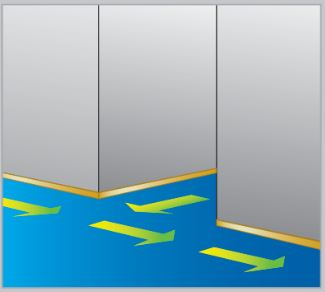
\includegraphics[width=\textwidth]{Figures/3. Lighting/light-safety8.jpg}
			\caption{Nas intersecções dos corredores}
			\label{fig: style 1 image h}
		\end{subfigure}
		\hfill
		\begin{subfigure}[b]{0.3\textwidth}
			\centering
			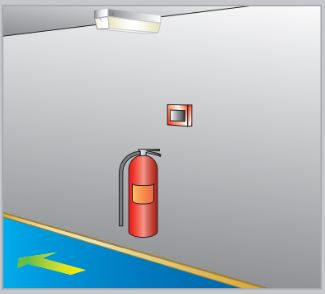
\includegraphics[width=\textwidth]{Figures/3. Lighting/light-safety9.jpg}
			\caption{Próximo a equipamentos de extinção de incêndio}
			\label{fig: style 1 image y}
		\end{subfigure}
		\caption{Localização das luminárias de emergência} fonte das imagens \cite{eaton2013} 
		\label{fig: safety-luminarires-places}
	\end{figure}


% Copy this to add more chapters
\subsection{Sistema de proteção contra descargas atmosféricas} \label{subsection: spda}

XXXXXXXXXXXXXXXXXXXXXXXXXXXXXXXXX

\subsubsection{Coberturas metálicas}

Apesar de muitas pessoas acharem que um telhado metálico "atrai" mais raios que um telhado de outro material, diversos estudos provaram que esta afirmação é uma enorme inverdade.

Devido ao fato das coberturas metálicas formarem uma blindadem da Gaiola de Faraday é possivel utilizar sua estrutura para ajudar a dissipar a energia de uma descarga atmosférica.

O projetista deverá atentar-se a espessura da cobertura metálica não ser inferior as indicadas na tabela \ref{table: espessura chapa}.

\begin{table}[ht]
	\rowcolors{2}{Tue-red!10}{white}
	\centering
	\caption{Espessura mínima das coberturas metálicas - fonte \cite{2015aterramento}}
	\begin{tabular}[t]{ccc}
		\toprule
		\color{Tue-red}\textbf{Nível de proteção}&\color{Tue-red}\textbf{Material da chapa}&\color{Tue-red}\textbf{Espessura da chapa(mínimo)}\\
		\midrule
		I a IV&Aço&4mm\\
		I a IV&Cobre&3mm\\
		I a IV&Alumínio&7mm\\
		I a IV&Zinco&7mm\\
		\bottomrule
	\end{tabular}
	\label{table: espessura chapa}
\end{table}


% Copy this to add more chapters
%\subsubsection{Generalidades} \label{lighting - generalidades}

\begin{enumerate}
	
	\item O projeto de iluminação deverá abranger, onde cabível, os seguintes sistemas:
	\begin{enumerate}
		\item Iluminação geral de interiores
		\item Iluminação externa
		\item Iluminação específica
		\item Iluminação de emergência
		\item Iluminação de sinalização e luz de obstáculos
		\item Iluminação cênica (quando esta for exigida)
	\end{enumerate}
	
	\item Não será aceita a utilização de eletrodutos de bitola menor que 3/4” de diâmetro para iluminação.
	
	\item Poderá ser considerada a instalação como previsão de reserva, eletrodutos com bitolas superiores às necessárias para as bitolas iniciais dos condutores ou eletrodutos vazios.
	
	\item O projeto deverá priorizar, sempre que possível, a utilização de luminárias energeticamente eficientes.
	
	\item O projeto sempre deverá priorizar a utilização de equipamentos e materiais facilmente encontrados no mercado.
	
	\item Deverá ser priorizada a utilização de luminárias na seguinte ordem:\label{light: tipo1}
	\begin{enumerate}
		\item Utilização de luminárias LED com lâmpadas TUBOLED modelo T5, dado que as lâmpadas são facilmente substituídas.

		\item Luminárias com lâmpadas LED (a lâmpada ou o conjunto de lâmpadas pode ser facilmente substituído);
		
		\item Luminárias LED (o conjunto de LEDs não pode ser substituído, entretanto o \textit{driver} pode ser substituído;
	\end{enumerate}

	\item Deverá ser evitada, entretanto poderá ser utilizada em casos excepcionais:\label{light: tipo2}
	\begin{enumerate} 
		
		\item Luminárias LED cujo conjunto de lâmpadas e driver não podem ser substituídos (a manutenção deverá trocar todo o conjunto em caso de defeito)		
	\end{enumerate}

	\item Casos que não se enquadrem nos itens \ref{light: tipo1} e \ref{light: tipo2}, a contratante deverá ser contatada para definir junto a contratada quais luminárias e lâmpadas serão utilizadas.

	
	\item O projeto de iluminação atenderá aos níveis de iluminamento necessários em cada ambiente de acordo com a NBR-8.995 e determinará o tipo de iluminação, número de lâmpadas por luminárias, número e tipo de luminária, detalhes de montagem, localização das luminárias, caixas de passagem e interruptores, caminhamento dos condutores e tipo para sua instalação. 
	
	\item Para o projeto de iluminação poderão ser adotados os valores mínimos dos níveis de iluminamento recomendados pelas NBR 8.995. O tipo de fonte luminosa e da luminária e a sua distribuição no local deverão ser harmonizados com os projetos de arquitetura e aprovados pela coordenação do desenvolvimento do projeto.
	
	\item \label{lighting: bitola minima} Para circuitos de iluminação, será adotado a bitola mínima de 2,5mm\textsuperscript{2} observando-se, entretanto, a diferenciação de cores nas respectivas fiações.
	
	\item As derivações para a alimentação das luminárias serão executadas utilizando-se cabos de cobre “PP” de 3 vias \#1,5mm\textsuperscript{2} devendo ser indicadas em nota e preferencialmente em detalhe de projeto;
	
	\item Em instalações aparentes deverá ser utilizada as linhas disponíveis da Wetzel como referência técnica para interruptores e tampas montados em conduletes de alumínio
	
	\item A contratante utiliza alguns modelos de luminária (interna, externa e pública) como padrão de referência técnica. O projetista deverá consultar o apêndice XXXXXX para obter estes modelos ou apresentar à Engenharia da contratante para aprovação os modelos com características similares que pretende utilizar no projeto.
	
	\item Ao dimensionar os eletrodutos de tomadas, os mesmos deverão ser dimensionados com bitola mínima de 3/4"%$\dfrac{3}{4}$"
\end{enumerate}

% Copy this to add more chapters
%\subsubsection{Iluminação de interiores}\label {section: iluminacao_interiores}
	\begin{enumerate}
		\item Para a correta localização das fontes luminosas, a contratada, sempre que possível disporá as luminárias de forma simétrica a fim de garantir um bom bom fator de uniformidade (vide exemplo na figura \ref*{fig: disposicao}). Quaisquer disposições em contrário, a fiscalização deverá ser consultada.
		\begin{figure}[H]
			\centering
			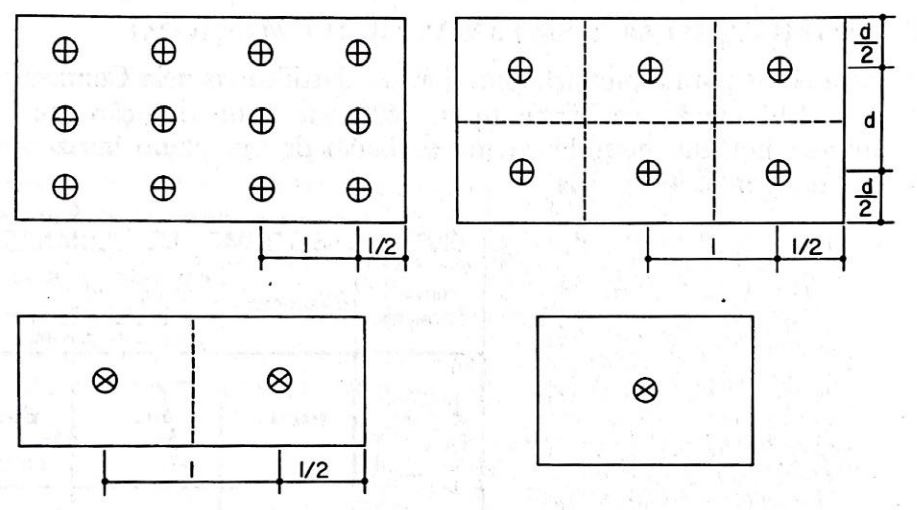
\includegraphics[width=\textwidth]{Figures/3. Lighting/light-disposicao.jpg}
			\hfill
			\caption{Disposição típicas de montagem para luminárias de iluminação de interior}  Referência \cite{de1987iluminação} p.112
			\label{fig: disposicao}
		\end{figure}
		
		\item Em instalações embutidas deverá ser utilizada a linha "PIALPLUS" da Legrand como referência técnica para interruptores e tampas
		
		\item Em instalações aparentes deverá ser utilizada a linha "Condulete TOP" da Tigre ou as linhas disponíveis da Wetzel como referência técnica para interruptores e tampas montados em conduletes de PVC
		
		\item Em instalações aparentes deverá ser utilizada as linhas disponíveis da Wetzel como referência técnica para interruptores e tampas montados em conduletes de alumínio
		
		\item\label{light:wc1}Em circuito de iluminação de banheiros e lavábulos será permitido conectar tomadas de uso geral (até 2 tomadas de 200W) ao referido circuito.
		
		\item\label{light:wc2}Em circuito de iluminação de banheiros e lavábulos será permitido conectar renovadores de ar do tipo "ventokit".
		
		\item Tomadas de uso geral não podem ser conectadas a circuitos de iluminação, a exceção das preconizadas nos itens \ref*{light:wc1} e \ref*{light:wc2}
		
		\item Em biotérios a contratada deverá prever um sistema de iluminação totalmente dimerizável
		
		\item Em Laboratórios NB3 ou NBA3 as luminárias dimensionadas serão do tipo herméricas
		\begin{enumerate}
			\item Laboratórios NB3 ou NBA3 com pavimento técnico a contratada deverá prever a remoção ou substituição dos equipamentos pelo referido pavimento, indicando em detalhe de projeto e notas
			\item Laboratórios NB3 ou NBA3 sem pavimento técnico e com forro de gesso, a contratada deverá prever em projeto que a face que possui o difusor da luminária irá facear o gesso e garantir a estanqueidade da área por sobre o gesso quando for necessário efetuar a manutenção da mesma.
			\item Demais casos deverão ser analisados pela contratada e discutidos com a Engenharia da COGIC.
		\end{enumerate}

		\item\label{light:encaixe10A}Nos caso dos encaixes rápidos utilizarem o conjunto tomada/plugue, deverá ser utilizada uma tomada de 10A
		
		\item As luminárias deverão ser projetadas tendo-se em mente a utilização de engate-rápido através de plugues e tomadas, ou dispositivos equivalentes, devendo a mesma ser indicada em nota e detalhada em projeto. Dois exemplos a seguir.
		
		\begin{figure}[H]
			\centering
			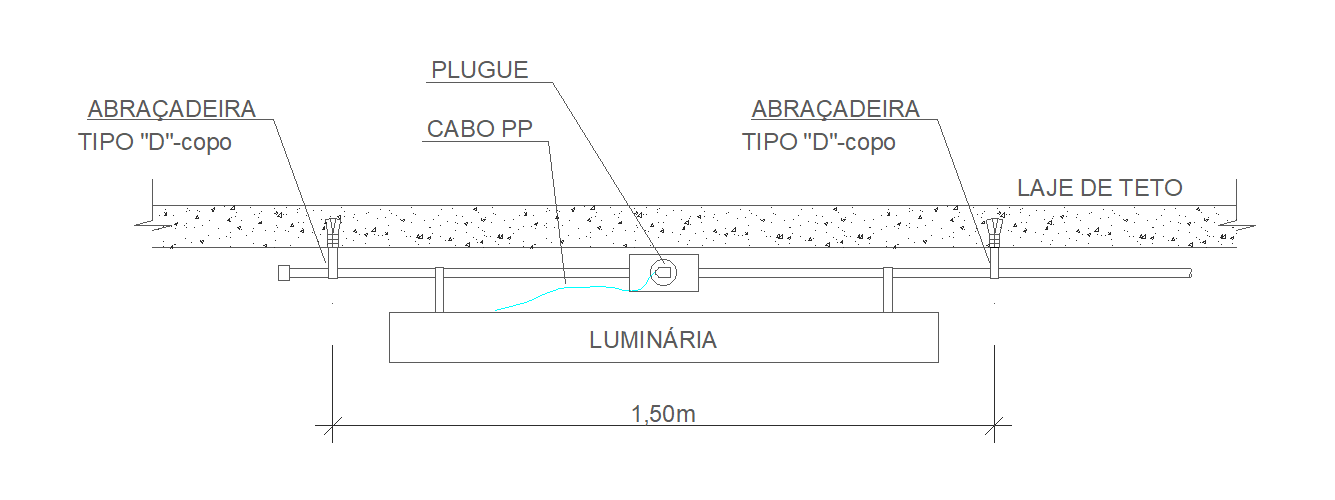
\includegraphics[width=\textwidth]{Figures/3. Lighting/light-engate rapido1.png}
			\hfill
			\caption{Encaixe rápido usando condulete e plugue de tomada ex.1}
			\label{fig: engate-rapido1}
		\end{figure}
		\begin{figure}[H]
			\centering
			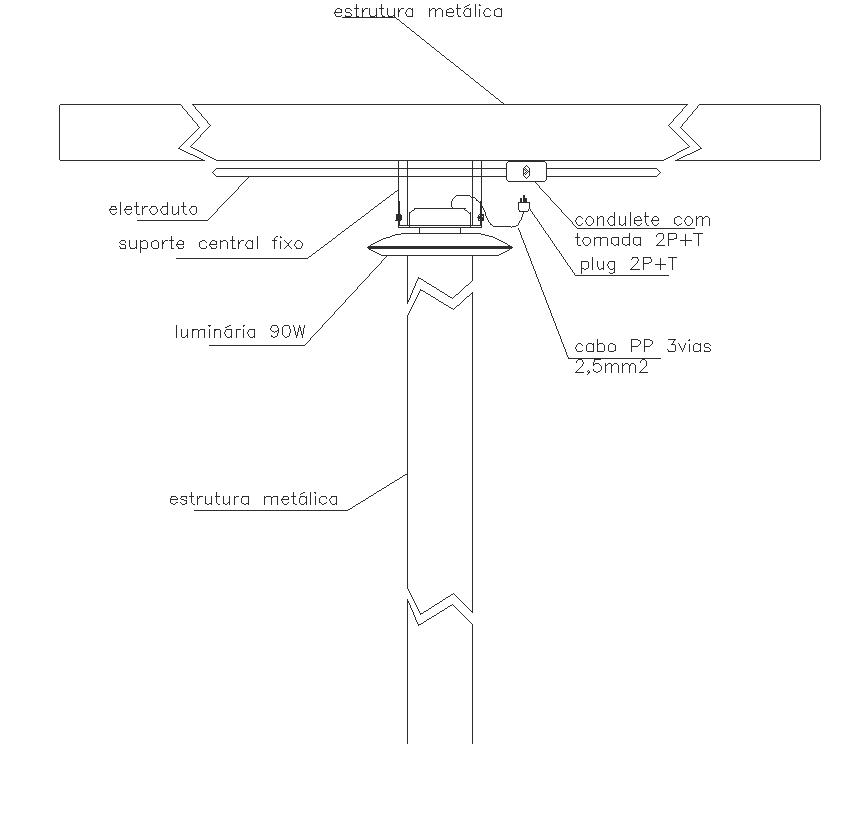
\includegraphics[scale=0.25]{Figures/3. Lighting/light-engate rapido2.png}
			\hfill
			\caption{Encaixe rápido usando condulete e plugue de tomada ex. 2}
			\label{fig: engate-rapido2}
		\end{figure}


		\item Luminárias instaladas em corredores deverão ser instaladas no sentido longitudinal a fim de obter um melhor rendimento no brilho e evitar ofuscamento. Melhores referências e explicações pode ser obtidas em \cite{simons2008lighting} p.74-75 e \cite{van2019interior} p.413.
		
		\item Luminárias em corredores só poderão ser instaladas no sentido transversal caso alguma exceção impossibilite a montagem no sentido longitudinal
	
	\end{enumerate}

% Copy this to add more chapters
%\subsubsection{Iluminação de emergência e sinalização de obstáculos}


	\paragraph*{Locais de instalação}
	
	Os locais específicos onde se fazem necessária a instalação de sinalização de emergência são:
	
	\begin{figure}[H]
		\centering
		\begin{subfigure}[b]{0.3\textwidth}
			\centering
			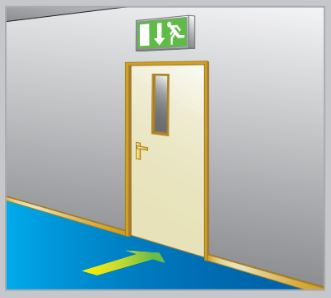
\includegraphics[width=\textwidth]{Figures/3. Lighting/light-safety1.jpg}
			\caption{A cada porta de emergência}
			\label{fig: style 1 image a}
		\end{subfigure}
		\hfill
		\begin{subfigure}[b]{0.3\textwidth}
			\centering
			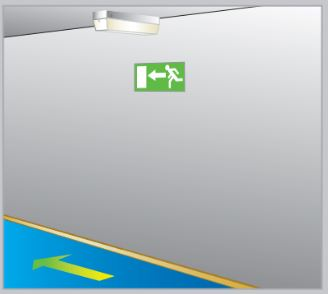
\includegraphics[width=\textwidth]{Figures/3. Lighting/light-safety2.jpg}
			\caption{Todas as sinalizações de saída}
			\label{fig: style 1 image b}
		\end{subfigure}
		\hfill
		\begin{subfigure}[b]{0.3\textwidth}
			\centering
			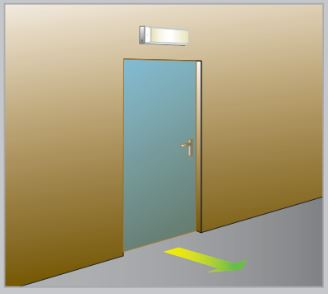
\includegraphics[width=\textwidth]{Figures/3. Lighting/light-safety3.jpg}
			\caption{Nas saídas de emergência}
			\label{fig: style 1 image c}
		\end{subfigure}
	\end{figure}

	\begin{figure}[H]
		\centering
		\begin{subfigure}[b]{0.3\textwidth}
			\centering
			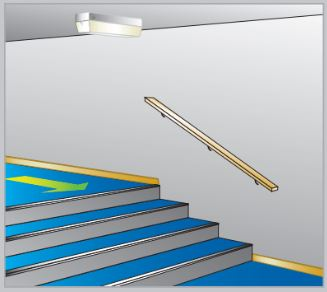
\includegraphics[width=\textwidth]{Figures/3. Lighting/light-safety4.jpg}
			\caption{Próximo escadas}
			\label{fig: style 1 image d}
		\end{subfigure}
		\hfill
		\begin{subfigure}[b]{0.3\textwidth}
			\centering
			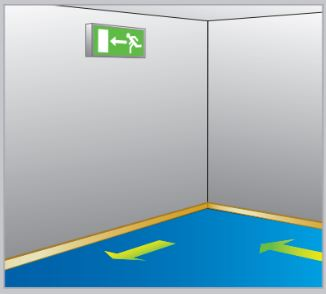
\includegraphics[width=\textwidth]{Figures/3. Lighting/light-safety5.jpg}
			\caption{Nas mudanças de direção}
			\label{fig: style 1 image e}
		\end{subfigure}
		\hfill
		\begin{subfigure}[b]{0.3\textwidth}
			\centering
			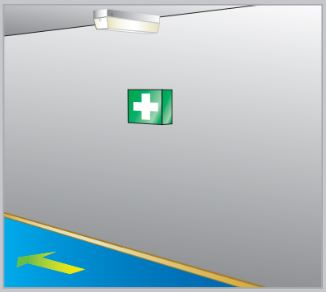
\includegraphics[width=\textwidth]{Figures/3. Lighting/light-safety6.jpg}
			\caption{Nos pontos de primeiro socorros}
			\label{fig: style 1 image f}
		\end{subfigure}
	\end{figure}

	\begin{figure}[H]
		\centering
		\begin{subfigure}[b]{0.3\textwidth}
			\centering
			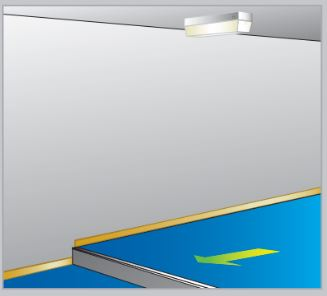
\includegraphics[width=\textwidth]{Figures/3. Lighting/light-safety7.jpg}
			\caption{A cada mudança de nível}
			\label{fig: style 1 image g}
		\end{subfigure}
		\hfill
		\begin{subfigure}[b]{0.3\textwidth}
			\centering
			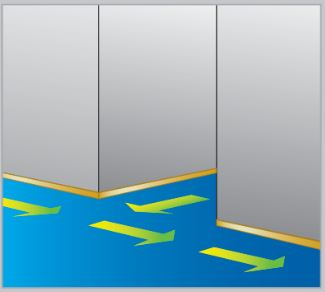
\includegraphics[width=\textwidth]{Figures/3. Lighting/light-safety8.jpg}
			\caption{Nas intersecções dos corredores}
			\label{fig: style 1 image h}
		\end{subfigure}
		\hfill
		\begin{subfigure}[b]{0.3\textwidth}
			\centering
			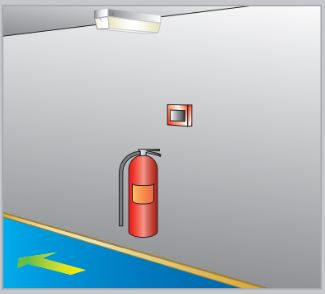
\includegraphics[width=\textwidth]{Figures/3. Lighting/light-safety9.jpg}
			\caption{Próximo a equipamentos de extinção de incêndio}
			\label{fig: style 1 image y}
		\end{subfigure}
		\caption{Localização das luminárias de emergência} fonte das imagens \cite{eaton2013} 
		\label{fig: safety-luminarires-places}
	\end{figure}

\newpage


\newpage
